\documentclass[pdftex]{article}
\usepackage[T1]{fontenc}
\usepackage[utf8]{inputenc}
\usepackage{graphicx}
\usepackage{caption}
\usepackage{titling}
\usepackage{enumitem}
\setlist[itemize]{leftmargin=*}
\setlist[description]{leftmargin=*}

\setlength{\droptitle}{-15em}
\title{PHYS 721 Homework 5}
\author{Nick Tyler}
\date{}


\begin{document}
\maketitle
\begin{enumerate}
	\item Three Breit-Wigner curves for the decay $\phi \rightarrow K^{+} K^{-}$ are fitted to data set 1. 
		The first fit, in green, is the relativistic Breit-Wigner with a mass dependent $\Gamma$, 
		$\Gamma = \Gamma_{0} \left( \frac{p}{p_0} \right)^3$. The second fit, in blue, is the relativistic Breit-Wigner. 
		The third fit, in red, is the Non-Relativistic Breit-Wigner curve. \

		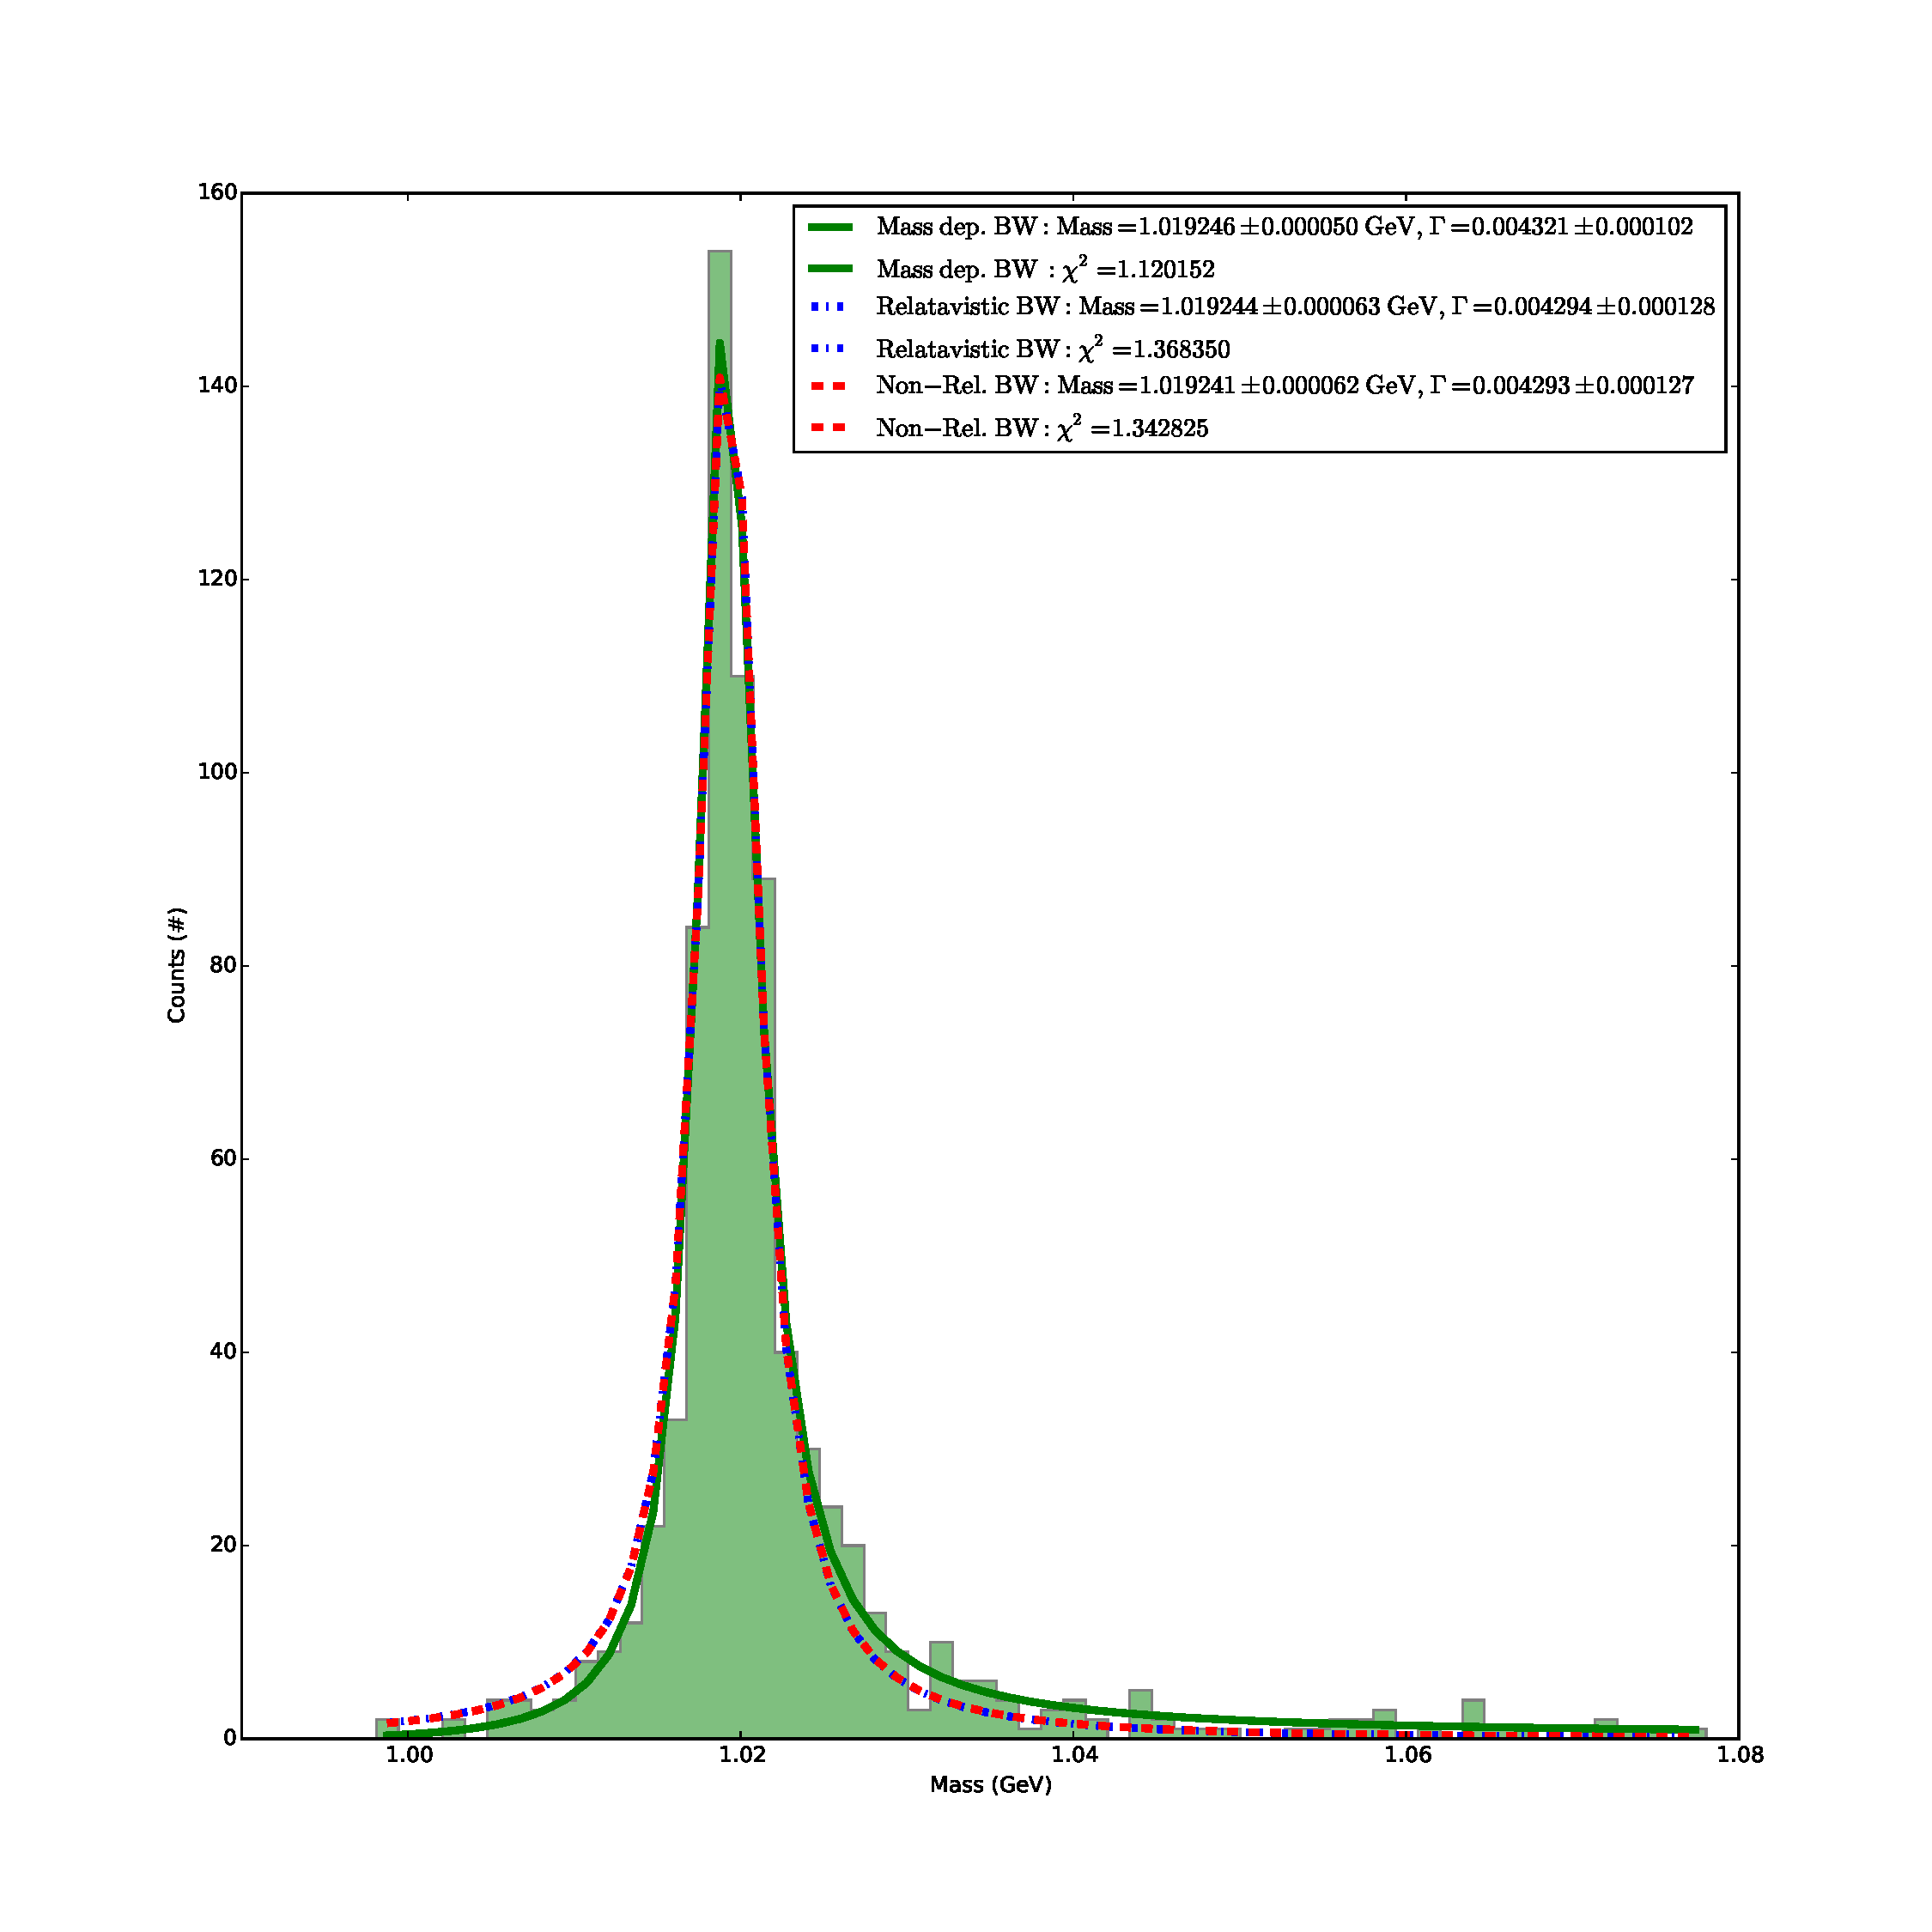
\includegraphics[scale=0.35]{Problem_1_and_2.pdf}\\
		\captionof{figure}{Three Breit-Wigner curves fit to data for, $\phi \rightarrow K^{+} K^{-}$}
		
	\pagebreak

	\item By looking at the $\chi^2$ values from figure one the first fit, the relativistic Breit-Wigner
		with mass dependent $\Gamma$ appears to give the best value because it's $\chi^2$ is closest to one.


	\item Stuff here for problem 3.
	\begin{center}
		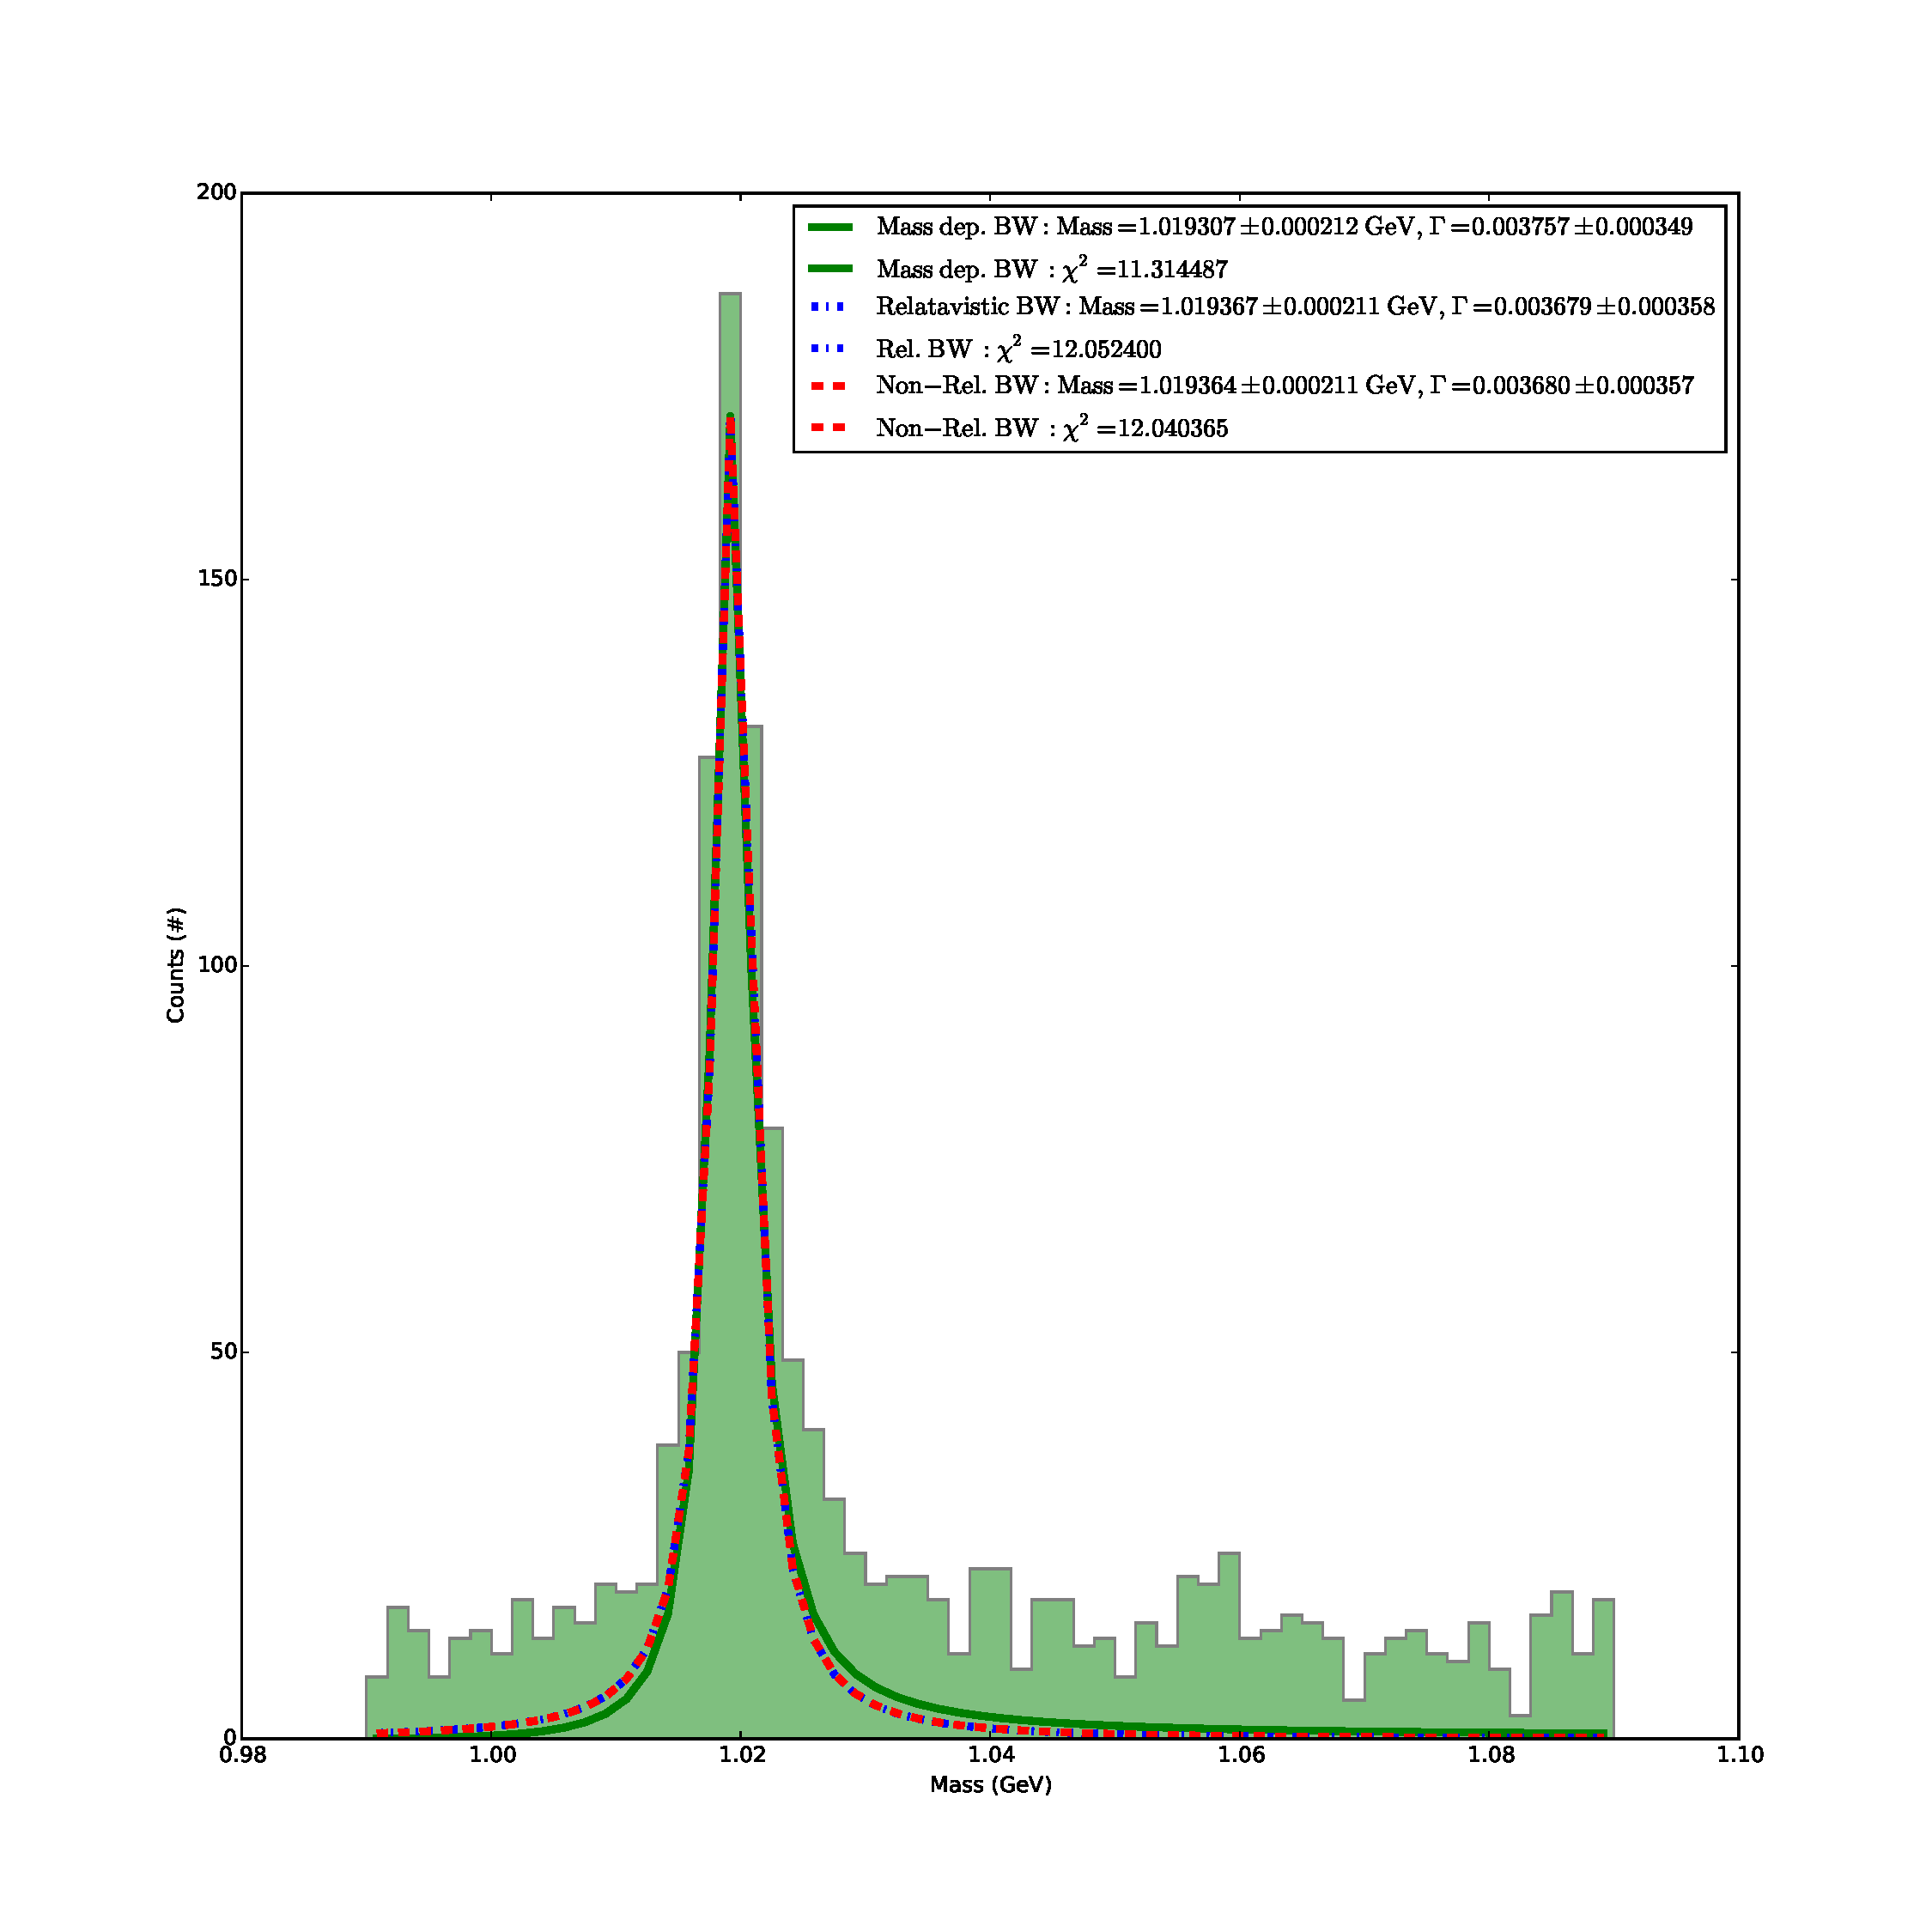
\includegraphics[scale=0.35]{Problem_3_nobackfit.pdf}
	\end{center}
		\captionof{figure}{Three Breit-Wigner curves with background fit to data for, $\phi \rightarrow K^{+} K^{-}$}
	\begin{center}
		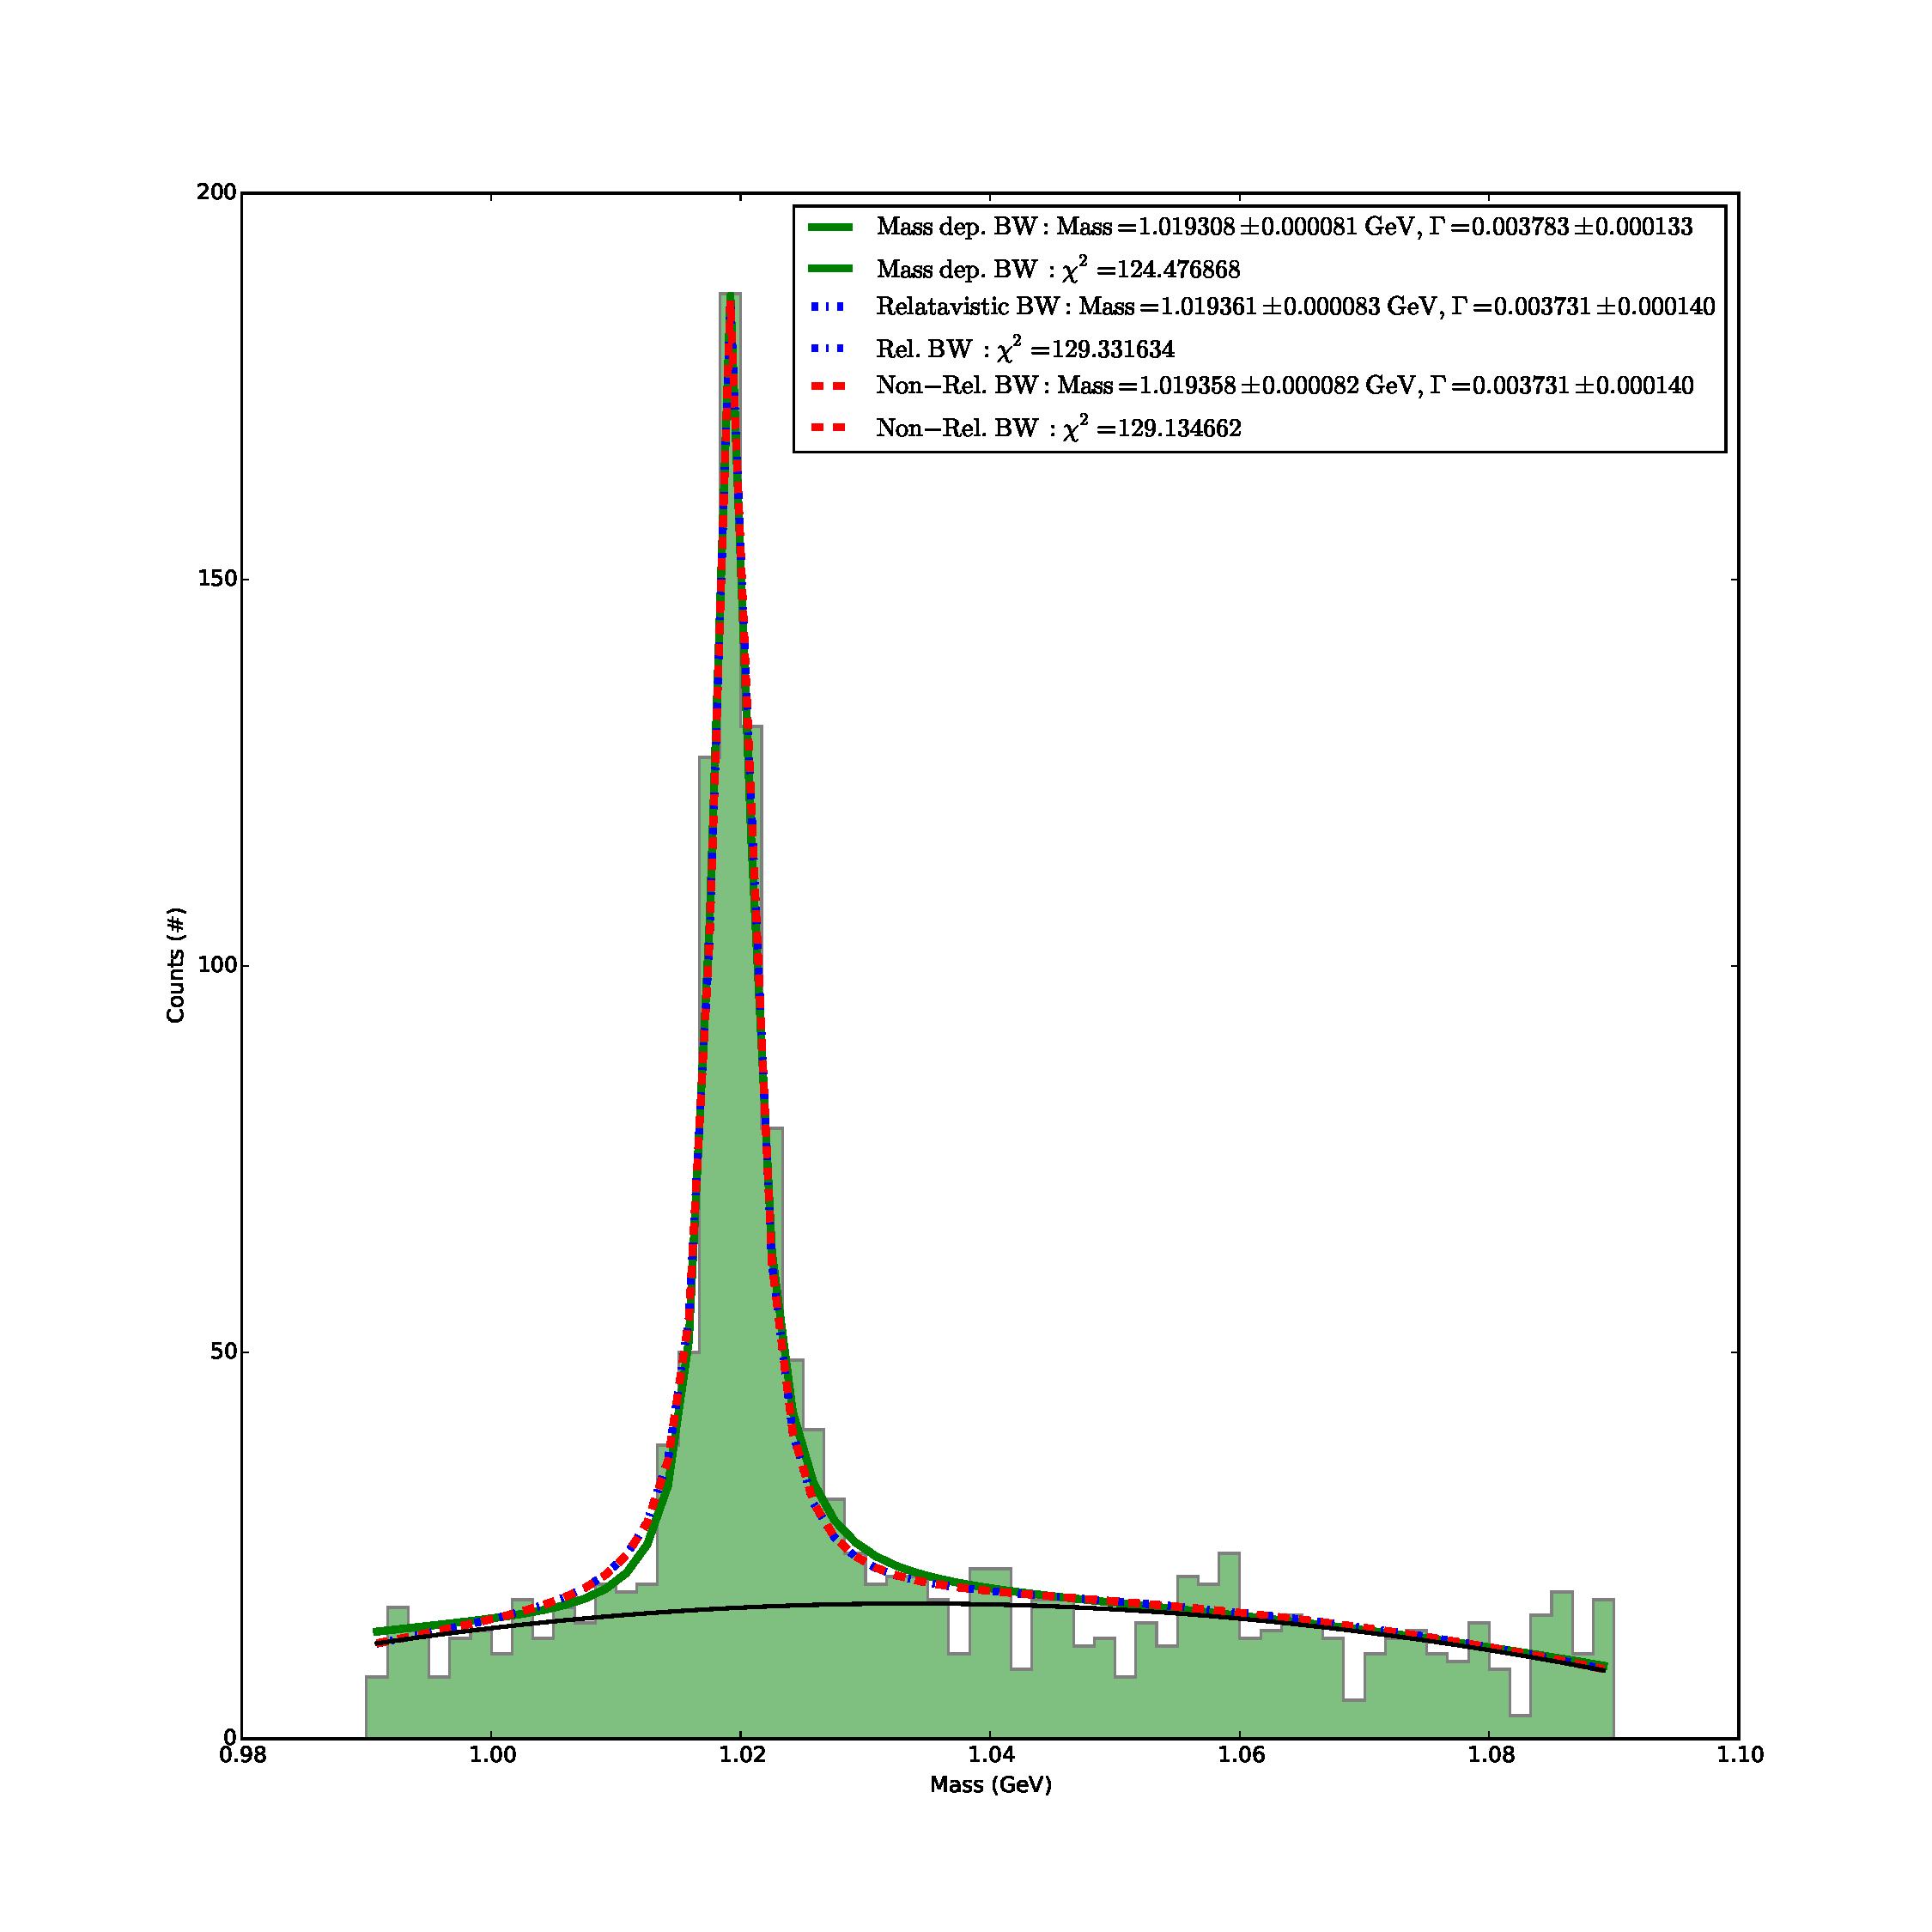
\includegraphics[scale=0.35]{Problem_3_withbackfit.pdf}
	\end{center}
		\captionof{figure}{Three Breit-Wigner curves with background fit with background for, $\phi \rightarrow K^{+} K^{-}$}

\end{enumerate}

\end{document}
